\section{Spectrum Estimation}
The problem of estimation a spectrum is, that there is never an infinity number of samples.
Therefore, the autocorrelation is always multiplied with a window.

\subsection{Nonparametric Method - Periodogram \hayes{393}}
\begin{tabbing}
autocorrelation: 	\= $\hat{r}_x(k) =\frac{1}{N} \sum \limits_{n=0}^{N-1-k} x(n+k)x^*(n)$   \hspace{4cm} \= $k=0,1,\ldots,N-1$ \\
power spectrum:  	\>  $\hat{P}_{per}(e^{jw}) = \frac{1}{N} X_N(e^{jw})X^*_N(e^{jw}) = $\\
\>					$\frac{1}{N}  \left\lvert X_N(e^{jw}) \right\rvert ^2 =  \frac{1}{N}  \left\lvert \sum\limits_{n=0}^{N-1} x(n)e^{-jn\omega} \right\rvert ^2$   \\
computing:  		\> The easiest way to compute the Periodogram is to compute the FFT, take the absolute values and square it\\
					\> $x_N(n) \xrightarrow{DFT} X_N(e^{jw}) \Rightarrow \frac{1}{N}  \left\lvert X_N(k) \right\rvert ^2 = \hat{P}_{per}(e^{j 2 \pi k/N})$ \\
Bias: 				\>  $E\left\lbrace \hat{P}_{per}(e^{jw}) \right\rbrace = \frac{1}{2 \pi}P_x(e^{jw})*W_B(e^{jw})$ \> $W_B$ $\to$ Bartlet window\\
Resolution: 		\>  $Res[\hat{P}_{per}(e^{jw})] = \Delta w = 0.89 \frac{2 \pi}{N}$\> Resolution = 3dB BW $(\Delta\omega)_{3dB}$\\
The Problem of the Periodogram is that the variance doesn't get smaller and it's far \textbf{too big!!!}.\\
Variance 			\> $Var\left\lbrace \hat{P}_{per}^{(i)}(e^{j\omega}) \right\rbrace \approx P^2_x(e^{j\omega})$\\
\end{tabbing}
Because the samples are multiplied with a rectangle window, a dirac in the original power spectrum becomes a sinc with a first sidelobe just 13 dB lower than the mainlobe.\\


The Periodogram is okay to be used when a high frequency resolution is required but should
not be used to estimate the spectrum accurately.

\subsection{Nonparametric Method - Modified Periodogram \hayes{408}}
To have a better sidelobe ratio, different windows are used to multiplied the given data.
\begin{tabbing}
autocorrelation: 	\= $\hat{r}_x(k) =\frac{1}{N} \sum \limits_{n=0}^{N-1-k} x(n+k)x^*(n)$   \hspace{4cm} \= $k=0,1,\ldots,N-1$ \\
power spectrum:  	\>  $\hat{P}_{M}(e^{jw}) = \frac{1}{NU}  \left\lvert \sum\limits_{n=\infty}^{\infty} w(n)x(n)e^{-jn\omega} \right\rvert ^2$   \\
scaling 			\> Because the window itself hasn't normaly a power of 1, the power spectrum has to be scaled by factor U:\\
\>					$U=\frac{1}{N} \sum\limits_{n=0}^{N-1}|w(n)|^2$\\
Bias: 				\>  $E\left\lbrace \hat{P}_{M}(e^{jw}) \right\rbrace = \frac{1}{2 \pi NU}P_x(e^{jw})*|W(e^{jw})|^2$\\
Resolution : 		\>  Window dependent\\
\textbf{The problem of variance isn't solved.}\\
Variance 			\> $Var\left\lbrace \hat{P}_{M}^{(i)}(e^{j\omega}) \right\rbrace \approx P^2_x(e^{j\omega})$\\
\end{tabbing}

\begin{minipage}{10cm}
\begin{tabular}{p{3cm} p{3cm} p{3cm}}
Window	 &  	Sidelobe 	&3dB BW\\
&				Level (dB)	& $(\Delta\omega)_{3dB}$\\
\hline
Rectangular&			-13	&		0.89 (2$\pi$/ N)\\
Bartlett (triangle)&	-27	&		1.28 (2$\pi$/ N)\\
Hann				&	-32	&		1.44 (2$\pi$/ N)\\
Hamming&				-43	&		1.30 (2$\pi$/ N)\\
Backman		&			-58	&		1.68 (2$\pi$/ N)
\end{tabular}
\end{minipage}
\begin{minipage}{8cm}
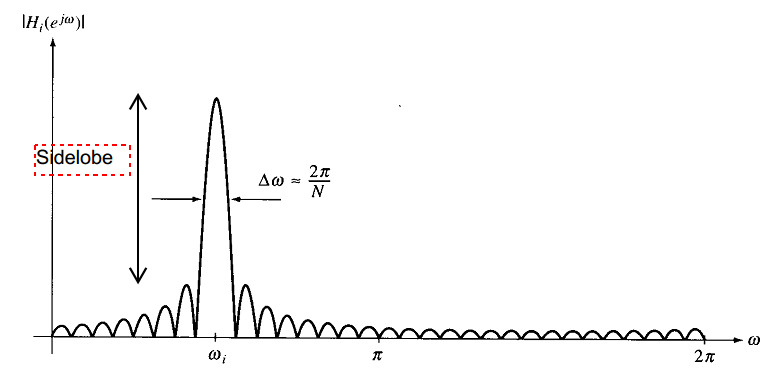
\includegraphics[width=8cm]{./bilder/sidelobe.jpg}
\end{minipage}





\subsection{Nonparametric Method - Bartlett's Method \hayes{412}}
The idea of Bartlett was to take $K$ non-overlapping sub-sequences (lenght $L$) of the given data.
A Periodogram (rectangular window) has to be calculated for every sub-sequence and then averaged. $N=K\cdot L$

\begin{tabbing}
power spectrum:  	\=  $\hat{P}_{B}(e^{jw}) = E\left\{\frac{1}{L}  \left|X_L(e^{jw})\right| ^2\right\} =  \frac{1}{N}\sum\limits_{i=0}^{K-1} \left|\sum\limits_{n=0}^{L-1} x(n+iL)e^{-jn\omega}\right| ^2$   \\
Bias: 				\>  $E\left\{ \hat{P}_{B}(e^{jw}) \right\} = \frac{1}{2 \pi}P_x(e^{jw})*W_B(e^{jw})$  \hspace{4cm} \= W $\to$ Bartlet window\\
Resolution: 		\>  $Res\left[\hat{P}_{B}(e^{jw})\right] = \Delta w = 0.89 \cdot K \cdot \frac{2 \pi}{N}$\> Resolution = 3dB BW $(\Delta\omega)_{3dB}$\\
Variance 			\> $Var\left\lbrace\hat{P}_{B}(e^{j\omega})\right\rbrace = \frac{1}{K} Var\left\lbrace \hat{P}_{per}^{(i)}(e^{j\omega}) \right\rbrace \approx \frac{1}{K}P^2_x(e^{j\omega})$\\
\end{tabbing}
So the problem of a bad and inconsistent variance could be eliminated. But the resolution is $K$ times worse.

\subsection{Nonparametric Method - Welch's Method \hayes{415}}
Welch' method is a modification of the Bartlett's method. It uses overlapping of the sub-sequences.
When maintaining $L$ = section length, $K$ = number of sections, $D$ = overlap, the formula
$\boxed{N=L+D(K-1)}$ can be established. This means, that if $D=L$ there is no overlap and $D=L/2$ means 50\% overlap.

\begin{tabbing}
Power spectrum:  	\=  $\hat{P}_{W}(e^{jw}) =  \frac{1}{KLU}\sum\limits_{i=0}^{K-1} \left|\sum\limits_{n=0}^{L-1} w(n) \cdot x(n+iD)e^{-jn\omega}\right| ^2$   \\
\>						$U = \frac 1L \sum\limits_{n=0}^{L-1}|w(n)|^2$ = equalization factor for the given window\\
Bias: 				\>  $E\left\lbrace \hat{P}_{W}(e^{jw}) \right\rbrace = \frac{1}{2 \pi LU}P_x(e^{jw})*|W(e^{jw})|^2$\\
Resolution: 		\>  Window dependent\\
Variance 			\> $Var\left\lbrace\hat{P}_{W}(e^{j\omega})\right\rbrace \approx \frac{9}{16} \frac{L}{N}P^2_x(e^{j\omega}) =
\frac{9}{16} Var\left\lbrace\hat{P}_{B}(e^{j\omega})\right\rbrace$ \qquad with Barlett window and 50\% overlap\\
\end{tabbing}


\subsection{Nonparametric Method - Blackman-Tukey \hayes{420}}
The idea of Blackman-Tukey is to minimize the effect of autocorrelation samples with a \em big lag\em, because with a finite data record the variance of $\hat{r_x}(k)$ will be large.
This is because these samples just have some few samples that can be averaged.
Therefore, the autocorrelation is weighted with a window (like Hann, Bartlett or Hamming).\\
The window length $M$ has to be much smaller than the length of the autocorrelation $N$: $M  \ll N \Rightarrow M < \frac{1}{5}N$
\begin{tabbing}
Power spectrum:  	\=  $\hat{P}_{BT}(e^{jw}) =  \sum\limits_{k=-M}^{M} \hat{r}_x(k)w(k)e^{-jk\omega} \qquad
						\hat{P}_{BT}(z) =  \sum\limits_{k=-M}^{M} \hat{r}_x(k)w(k)z^{-k}$   \\
Bias: 				\>  $E\left\lbrace \hat{P}_{BT}(e^{jw}) \right\rbrace = \frac{1}{2 \pi}P_x(e^{jw})*W(e^{jw})$  \hspace{2cm} \= W $\to$ choosen window\\
Resolution: 		\>  Winow dependent\\
Variance 			\> $Var\left\lbrace\hat{P}_{BT}(e^{j\omega})\right\rbrace \approx P^2_x(e^{j\omega}) \frac{1}{N} \sum\limits_{k=-M}^{M}w^2(k)$\\
\end{tabbing}

\subsection{Performance Comparison \hayes{424}}
To compare different methods the following criteria can be used:\\
\begin{tabbing}
Variability:   \hspace{1cm}  	\=
  $\nu=\frac{Var\left\lbrace\hat{P}_{x}(e^{j\omega})\right\rbrace}{E^2\left\lbrace\hat{P}_{x}(e^{j\omega})\right\rbrace}=\frac{\sigma^2}{\mu^2}$
  \hspace{1cm} \= it's also called normalized variance (smaller is better)\\
  resolution \> $\Delta \omega$ \> smaller is better\\
  figure of merit					\> $M=\nu\cdot \Delta\omega$ \> smaller is better\\
\end{tabbing}
\begin{tabular}{p{3cm} | p{2cm} p{2.5cm} p{3cm}}
& Variability & Resolution & Figure of Merit\\
& $\nu$	&	$\Delta\omega$	& M \\
\hline\\
Periodogram & 1 & $0.89 \frac{2\pi}{N}$ & $0.89 \frac{2\pi}{N}$\\\\
Bartlett & $\frac{1}{K}$ & $0.89\cdot K \cdot  \frac{2\pi}{N}$ & $0.89 \frac{2\pi}{N}$\\\\
Welch & $\frac{9}{8\cdot K}$ & $1.28 \frac{2\pi}{L}$ & $0.72 \frac{2\pi}{N}$\\\\
Blackman-Tukey (Barlett)& $\frac{2\cdot M}{3\cdot N}$  & $0.64 \frac{2\pi}{M}$ & $0.43 \frac{2\pi}{N}$
\end{tabular}

\subsection{Parametric Method - Minimum Variance Method \hayes{426}}
Power spectrum: $\hat{P}_{MV}(e^{jw}) = \frac{p+1}{e^H R_x^{-1}e} \quad R_x = \text{Autocorrelation Matrix} \quad e=[1,e^{j\omega},\ldots, e^{jp\omega}]^T$

\subsection{Parametric Method - Maximum Entropy Method \hayes{433}}
The idea is to use a infinite autocorrelation. For that we have to interpolate the missing samples.
The maximum entropy method (MEM) uses an all pole interpolation.
Because of this, the MEM is really good \textbf{if and only if} the spectrum of an \textbf{all-pole model} is given.
The coefficients $a_p(k)$ are calculated using the autoregressive model method described in section \ref{sec:autoregressive_model_method}.

\begin{tabbing}
Power spectrum:  	\=  $\hat{P}_{MEM}(e^{jw}) =  \frac{|b(0)|^2}{\left| 1 + \sum\limits_{k=1}^{p} a_p(k)e^{-jk\omega}\right|^2} =
						\frac{|b(0)|^2}{\left|e^H a_p\right|^2}$
						\hspace{1cm} \= $a_p=[1,a_p(1),\ldots, a_p(k)]^T \quad e=[1,e^{j\omega},\ldots, e^{jp\omega}]^T $ \\
\>						$\epsilon_p = |b(0)|^2 = r_x(0) + \sum\limits_{k=1}^p a_p(k) r_x^*(k)$ \\
\end{tabbing}
